\documentclass[compress,dvipsnames]{beamer}

\usepackage[orientation=portrait, size=a0, scale=1.0, debug]{beamerposter}
\usepackage[english]{babel}
\usepackage[latin1, utf8]{inputenc}
\usepackage{transparent}
\usepackage{svg}
\usepackage{shellesc}
\usepackage{tikz}
\usepackage{listings}
\usepackage{authoraftertitle}

\newcommand{\mainRuleThickness}{4pt}
\newcommand{\contentRuleTickness}{3pt}
\newcommand{\columnWidth}{0.485}
\newcommand{\timeTitleSize}{\LARGE}
\newcommand{\blockTitleSize}{\huge}
\newcommand{\EM}{EMail}
\newcommand{\EMs}{EMails}
\newcommand{\Em}{email} % Not using \em, because this command is already defined!
\newcommand{\Ems}{emails}
\newcommand{\Ph}{Phishing}
\newcommand{\ph}{phishing}
\newcommand{\phm}{phishing mail}
\newcommand{\phms}{phishing mails}
\newcommand{\Phm}{Phishing mail}
\newcommand{\Phms}{Phishing mails}
\newcommand{\iconHeight}{3.0cm}
\newcommand{\iconWidth}{\iconHeight}
\newcommand{\transparentLevel}{0.75}

\usetheme{default}

\setbeamercolor{background canvas}{bg=gray!5}
\setbeamercolor{block title}{bg=blue!15,fg=black}

\title{The evolution of \Phm s}
\author{}
\date{\today}

\graphicspath{{./}{./Pics}}



%%%%% %%%%% %%%%% %%%%% %%%%% BEGIN document %%%%% %%%%% %%%%% %%%%% %%%%%
\begin{document}
% Remove navigation bar of beamer templates
\beamertemplatenavigationsymbolsempty

\phantom{X}
% Title box
\begin{block}
    {\phantom{X}\\\centering \textbf{\Huge\inserttitle}\\\phantom{X}}
\end{block}

% \rule[0cm]{\textwidth}{\mainRuleThickness}

\begin{block}{\centering \blockTitleSize Introduction}
    \begin{columns}[T]
        \begin{column}{0.485\textwidth}
            \begin{minipage}[t][0.075\textheight][t]{\textwidth}
                \large
                \emph{An \Em\space is not a secure communication method.} This is an advice given from global companies like Google and also from governments across the world.

                The underlying technology was \textbf{designed in the 80s} [1]. Back in this time, there was no widely available encryption or authentication; so both of this security aspects were not considered much.
            \end{minipage}
        \end{column}

        \begin{column}{0.485\textwidth}
            \begin{minipage}[t][0.075\textheight][t]{\textwidth}
                \large
                The lack of authentication makes it possible, that everyone can send fraud \Ems\space that appear to be from a trusted source, such as a government agency or a bank. Such an attack is called \ph. This is, as of 2020, most common type of cybercrime [2]. This poster summarizes the evolution of \phm s back from the beginning to today and provides information on how to recognize \phm s and whether the situation will improve in the future
            \end{minipage}
        \end{column}
    \end{columns}
\end{block}

\vspace{-1.5cm}
\rule[0cm]{\textwidth}{\mainRuleThickness}
\phantom{X}\\
{\large \textbf{HISTORY OF PHISHING MAILS}}
% \vspace{-2cm}


% Timeline with events
\newcommand{\up}{1}
\newcommand{\down}{-1}
% The number of timeline entries must be known and adjust manually, because the last entry in the data has problems in the usage of colors with macro replacements. I don't know why ... This is a simple (but not user-friendly) workaround
\newcommand{\numOfTimelineEntries}{9}
\begin{tikzpicture}[very thick, black]

% Coordinates
\coordinate (Origin) at (-1cm, 0cm); % Origin
\coordinate (End) at (80cm, 0cm); % End

% Timeline arrow
\draw [->, line width=0.15cm] (Origin) -- (End);

\foreach \year/\yearPos/\updown/\rectWidth/\rectHeight/\timelineDistance/\text/\c [count = \i]
in
{
    % The color of the last entry will be ignored and a hard coded color is used to avoid problems with the text repacements
    1987/7.5/\up/11.5/7/7/The first \ph\space attack cannot be determined exactly. A paper by the International HP Users Group\, Intertex\, described the general technique already in 1987 [3]./CornflowerBlue!50,
    1994/15/\down/11/6/4/The first documentated broader \ph\space attack was done with the software AOHell. At least 20.000 victims were affected [4]./Yellow,
    1995/18/\up/7/3.25/4.5/First recorded mention of the term \emph{\ph} [4]/YellowGreen!50,
    2001/28/\down/12/6/3/Rise of e-commerce due to the dot-com bubble. \emph{Spoofed websites} (fake websites) from popular domains like PayPal or eBay become mainstream./BurntOrange!75,
    $\thickapprox$2004/35/\up/12.5/6/5/\emph{Spear \ph} (targeted \ph) was invented. Before sending a mail a research of the victim will be done to construct a legitimate looking mail./PineGreen!25,
    2008/45/\down/11/6/6/Bitcoin and other cryptocurrencies were launched. Now a complete anonymous payment for recieving money from victims is possible./Tan!75,
    2013/52.5/\up/8.5/4/3/\Ph\space becomes the main technique to deliver ransomware./Goldenrod!50,
    2016/62/\down/12.5/5.5/4/Political topics become targets. \Ph\space was used for political influence in the USA election campain with the hacked account of John Podesta. [5]/Emerald!50,
    2020/70/\up/10/4.5/5/Fake \Ems\space from authorities (especially health authorities) were sent on a massive scale. [6]/Black
}
{
    % Year label
    \node at (\yearPos, \updown) {\textbf{\year}};

    % Line from timeline to box
    \draw [<-, ultra thick] (\yearPos, 0) -- (\yearPos, {\timelineDistance * \updown * -1});

    % Box with text
    % The positon information must be calculated
    \ifnum \updown = \down
        \ifnum \i < \numOfTimelineEntries
            \draw [fill=\c] ({\yearPos - (\rectWidth * 0.5)}, {\rectHeight + \timelineDistance * \updown * -1}) rectangle ({\yearPos + (\rectWidth * 0.5)}, {\timelineDistance * \updown * -1}) node[midway, align=center, text width = {\rectWidth cm * 0.9}] {\text};
        \else
            \draw [fill=Salmon!40] ({\yearPos - (\rectWidth * 0.5)}, {\rectHeight + \timelineDistance * \updown * -1}) rectangle ({\yearPos + (\rectWidth * 0.5)}, {\timelineDistance * \updown * -1}) node[midway, align=center, text width = {\rectWidth cm * 0.9}] {\text};
        \fi
    \else
        \ifnum \i < \numOfTimelineEntries
            \draw [fill=\c] ({\yearPos-(\rectWidth * 0.5)}, {\timelineDistance * \updown * -1}) rectangle ({\yearPos+(\rectWidth * 0.5)}, {\timelineDistance * -1 + \rectHeight * \updown * -1}) node[midway, align=center, text width = {\rectWidth cm * 0.9}] {\text};
        \else
            \draw [fill=Salmon!40] ({\yearPos-(\rectWidth * 0.5)}, {\timelineDistance * \updown * -1}) rectangle ({\yearPos+(\rectWidth * 0.5)}, {\timelineDistance * -1 + \rectHeight * \updown * -1}) node[midway, align=center, text width = {\rectWidth cm * 0.9}] {\text};
        \fi
    \fi
}

% Add icons
\node () at (4, 2) {\transparent{\transparentLevel}
\includegraphics[width=\iconWidth, height=\iconHeight]{45176_crt_monitor_icon.png}};
\node () at (10, -2) {\transparent{\transparentLevel}\includesvg[width=\iconWidth, height=\iconHeight]{Oxygen480-actions-document-save.svg}};
\node () at (20, -2) {\transparent{\transparentLevel}
\includegraphics[width=\iconWidth, height=\iconHeight]{3840px-Microsoft_Windows_95_logo_with_wordmark_cutted.svg.png}};
\node () at (32.5, -2) {\transparent{\transparentLevel}\includesvg[width=\iconWidth, height=\iconHeight]{CD_icon_test.svg}}
\node () at (42.5, 2) {\transparent{\transparentLevel}
\includegraphics[width=\iconWidth, height=\iconHeight]{Microsoft_Windows_XP_Logo_2_cutted.svg.png}}
\node () at (47.5, 2) {\transparent{\transparentLevel}\includesvg[width=\iconWidth, height=\iconHeight]{19_icon-icons.com_73780.svg}}
\node () at (67.5, -2) {\transparent{\transparentLevel}\includesvg[width=\iconWidth, height=\iconHeight]{cloud-upload_icon-icons.com_54314.svg}}
\node () at (73.5, 2) {\transparent{\transparentLevel}
\includegraphics[width=\iconWidth, height=\iconHeight]{Windows_11_logo_cutted.svg.png}}
\end{tikzpicture}

\phantom{X}\newline
\rule[1cm]{\textwidth}{\mainRuleThickness}

\begin{block}{\centering\blockTitleSize Examples of real \ph\space mails}
    \begin{columns}
        \begin{column}{\columnWidth\linewidth}
            \begin{figure}[h]
                \begin{tikzpicture}
                    \node (screenShot) at (0,0) {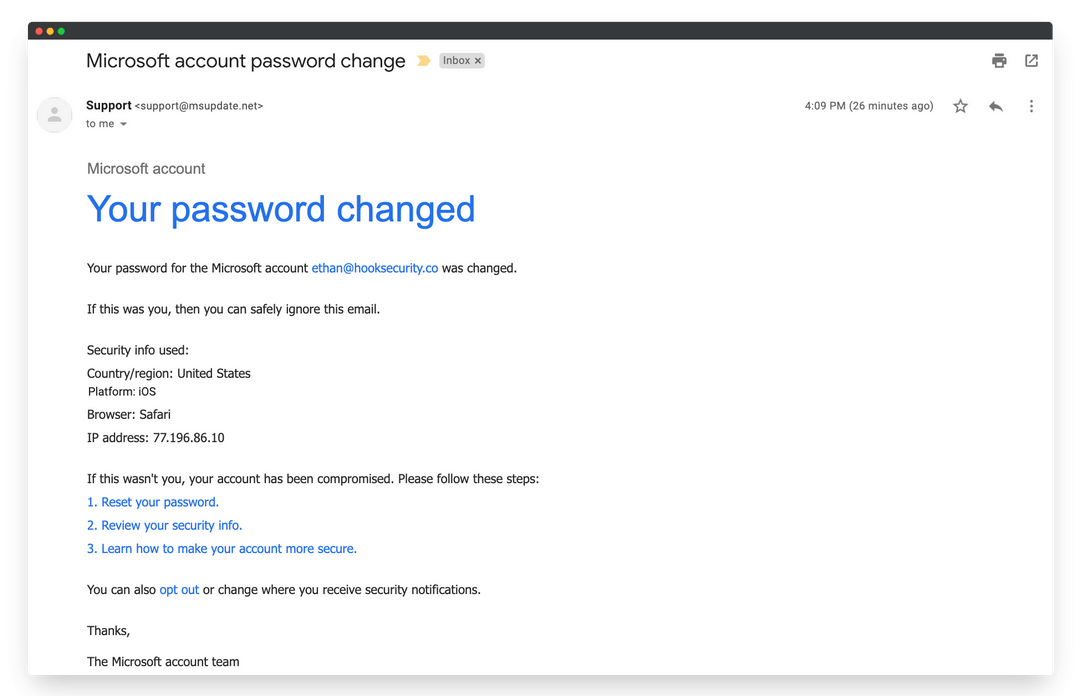
\includegraphics[scale=1.0]{60132635dca98cce734c23bb_microsoft-p-1080.png}};
                    \draw [red, ultra thick] (-12.5, 8.9) rectangle (-9.5, 8.15);
                    \draw [->, red, line width=0.15cm] (-7.5, 7.15) -- (-9.4, 8.1);
                    \node [right, red] at (-7.5, 7.15) {Wrong domain! \emph{microsoft.com} is correct};
                \end{tikzpicture}
                \caption{Microsoft \ph\space mail $\thickapprox$2018 [7].}
            \end{figure}
        \end{column}
        \begin{column}{\columnWidth\linewidth}
            \begin{figure}[h]
                \begin{tikzpicture}
                \coordinate (test) at (0, 10);

                \node at (0, 0) {
                \begin{lstlisting}
> *From:* Google <no-reply@accounts.googlemail.com>
> *Date:* March 19, 2016 at 4:34:30 AM EDT
> *To:* xxxxxxx@gmail.com
> *Subject:* *Someone has your password*
>
> Someone has your password
> Hi John
>
> Someone just used your password to try to sign in to your Google Account
> xxxxxxx@gmail.com.
>
> Details:
> Saturday, 19 March, 8:34:30 UTC
> IP Address: 134.249.139.239
> Location: Ukraine
>
> Google stopped this sign-in attempt. You should change your password
> immediately.
>
> CHANGE PASSWORD <https://bit.ly/1PibSU0>
>
> Best,
> The Gmail Team
> You received this mandatory email service announcement to update you about
> important changes to your Google product or account.
\end{lstlisting}
};
\draw [red, ultra thick] (-10, -8) rectangle (2, -6.85);
\draw [->, red, line width=0.15cm] (7.5, -5.85) -- (2.5, -6.85);
\node [right, red] at (7.5, -5.85) {Shortend link!};

\draw [red, ultra thick] (-1, 13) rectangle (6.5, 12);
\draw [->, red, line width=0.15cm] (7.5, 10) -- (6.5, 11.75);
\node [right, red, align=center] at (7.5, 8.75) {Wrong domain! \emph{google.com}\\is correct};
\end{tikzpicture}
                \caption{The John Podesta \Em leaked by WikiLeaks in 2016 [5].}
            \end{figure}
        \end{column}
    \end{columns}
\end{block}

\rule[0cm]{\textwidth}{\mainRuleThickness}
\vspace{1cm}

\begin{block}{\centering \blockTitleSize Tipps to identify \phms}
    \begin{columns}[T]
        \begin{column}{0.485\textwidth}
            \begin{minipage}[t][0.1\textheight][t]{\textwidth}
                \large
                \begin{itemize}
                    \item Subtle misspellings in the sender's address
                    \begin{itemize}
                        \large
                        \item "g\textbf{00}gle.com" instead of "g\textbf{oo}gle.com"
                        \item "microsof\textbf{f}.com" instead of "microsof\textbf{t}.com"
                    \end{itemize}
                    \item Unfamiliar greetings or missing name in the greeting ("Hi", "Hello", "Dear customer")
                    \item Grammar and spelling mistakes
                \end{itemize}
            \end{minipage}
        \end{column}

        \begin{column}{0.485\textwidth}
            \begin{minipage}[t][0.075\textheight][t]{\textwidth}
                \large
                \begin{itemize}
                \item Creating time pressure
                    \begin{itemize}
                        \large
                        \item "Your account will be suspended in the next few days"
                        \item "Action required"
                    \end{itemize}
                    \item Requesting for personal information
                    \beg
                    \item Unusual file types in the attachment (e.g. ".exe", ".bat", ".java")
                \end{itemize}
            \end{minipage}
        \end{column}
    \end{columns}
\end{block}

\vspace{-3cm}

\begin{block}{\centering \blockTitleSize Conclusion}
    \begin{columns}[T]
        \begin{column}{0.485\textwidth}
            \begin{minipage}[t][0.075\textheight][t]{\textwidth}
                \large
                If \Em\space were developed today, the technical design would be completely different. Nevertheless, despite its technical problems, \Em\space will not lose its importance. Because although we are now more networked than ever, we are also more fragmented than ever. Sending a message from one messenger service to another is not possible. The same applies to the countless social media platforms. Email is the only generally accepted technology that works across platforms. \emph{This technology is not good, but it's the best we have.}
            \end{minipage}
        \end{column}

        \begin{column}{0.485\textwidth}
            \begin{minipage}[t][0.075\textheight][t]{\textwidth}
                \large
                If current trends continue, the number of \phms\space will continue to increase. And recognizing them will also become increasingly difficult. Not least due to the constant development of large language models.\\

                \large
                \textbf{The problem with \phms\space cannot be solved technically in practice. The only possibility that exists is education!}
            \end{minipage}
        \end{column}
    \end{columns}
\end{block}

\rule[0cm]{\textwidth}{\mainRuleThickness}

\phantom{X}\\
REFERENCES
\begin{columns}[T]
    \begin{flushleft}
        \begin{column}{0.875\textwidth}
            \begin{minipage}[t]{0.85\textwidth}
                \begin{enumerate}
                    \item \url{https://datatracker.ietf.org/doc/html/rfc821}
                    \item \url{https://www.ic3.gov/Media/PDF/AnnualReport/2020_IC3Report.pdf}
                    \item Felix, Jerry \& Hauck, Chris (September 1987). "System Security: A Hacker's Perspective". 1987 Interex Proceedings. 8: 6.
                    \item \url{https://web.archive.org/web/20051214053144/http://wired-vig.wired.com/news/technology/0\%2C1282\%2C9932\%2C00.html}
                    \item \url{https://www.cbsnews.com/news/the-phishing-email-that-hacked-the-account-of-john-podesta/}
                    \item \url{https://www.bka.de/SharedDocs/Kurzmeldungen/DE/Warnhinweise/200507_Coronaphishing.html}
                    \item \url{https://www.hooksecurity.co/phishing-examples/microsoft-phishing-example}
                \end{enumerate}
            \end{minipage}
        \end{column}
        \hspace{0.75cm}
        \vline
        \hspace{0.75cm}
        \begin{column}{0.125\textwidth}
            \begin{minipage}[t]{0.85\textwidth}
                \vspace{-0.75cm}
                
\includegraphics[scale=0.075]{QR_Code_Git_Link.png}

                Created with \LaTeX\\
                Get the source code via this QR code.
            \end{minipage}
        \end{column}
    \end{flushleft}
\end{columns}

\end{document}
%%%%% %%%%% %%%%% %%%%% %%%%% END document %%%%% %%%%% %%%%% %%%%% %%%%%
